\chapter{Bitcoin system}

\section{Basic requirements for a banking system}

In any currency/banking system, there are some basic requirements that the system must provide. We list them here:
\begin{enumerate}
    \item There should be a unit of currency/money.
    \item There should be a standard way of keeping accounts, i.e., keeping track of how much money each person owns, and transferring money between accounts.
    \item No user should be able to create new money from thin air. Put differently, there should be a
    fixed amount of money in the system at any given time, and new money should be introduced in a systematic manner.
    \item A user should not be able to spend more money than he/she owns. There should be a way to verify whether or not this happens.
    \item One user should not be able to spend someone else’s money (at least, not without their permission).
     
\end{enumerate}
Let us see how the Bitcoin system provides these features.

\section{Bitcoin and Satoshi}
\begin{enumerate}
    \item The basic unit of currency in the Bitcoin system is Bitcoin, and the smallest denomination is called a Satoshi, which is equal to $10^{-8}$ Bitcoins.
    \item All transactions in Bitcoin must be an integer multiple of a Satoshi.
    \item Just like other currencies, there is an exchange rate between Bitcoin and the dollar. As of July 22, 2023, one Bitcoin is worth 30,000 US dollars. However, the exchange rate between Bitcoin and dollars is very volatile due to various factors, including greed and speculation.
    \item The classification of Bitcoin as a currency (like the US Dollar) or a store of value (like gold) has been widely debated. The mainstream view is that Bitcoin is a combination of both.
    \item Economically valuing Bitcoin, both in the short and long terms, is an active area of research.
    \item Understanding the economic aspects of Bitcoin, both as a currency and a store of value, involves studying various aspects of the Bitcoin system.
\end{enumerate}

\section{Transactions}
In ordinary parlance, the term \textbf{transaction} refers to an exchange of something of value. In the context of Bitcoin and cryptocurrencies, a transaction is simply a message that specifies the transfer of money from one entity to another. Transactions are the data values that get recorded on the blockchain. The blockchain as a ledger is therefore an ordered list of transactions. From this publicly verifiable ledger, any user can detect whether transactions are made according to certain rules or not, thereby lending credibility to the ledger and the currency.
\subsection{Addressing}
\begin{enumerate}
    \item \textbf{Bitcoin Address and Its Generation:}
    \begin{itemize}
        \item In Bitcoin, the notion of traditional accounts is replaced with addresses.
        \item An address is simply the hash of a user's public key. It is a unique alphanumeric string that serves as a destination for receiving bitcoins.
        \item Addresses are also used to determine where bitcoins will be sent in a transaction.
        \item New pairs of public and private keys, and thus new addresses, can be generated at will by a single user.
    \end{itemize}
    \item \textbf{Receiving vs. Spending Coins:}
    \begin{itemize}
    \item To receive coins, a user only needs to share their Bitcoin address with others. The address serves as a public identifier for receiving funds.
    \item However, to spend coins, a user must also reveal the corresponding public key associated with the address.
    \item This is because spending requires providing proof of ownership through a digital signature, which is created using the user's private key.
    \item The idiosyncrasy lies in the fact that while an address (hash of the public key) is publicly visible and used for receiving the associated public key is only revealed during the spending process for cryptographic verification.
    \end{itemize}
\end{enumerate}
\subsection{Transaction inputs and outputs}
\begin{enumerate}
    \item \textbf{Transaction Inputs:} 
    \begin{itemize}
        \item Each transaction input represents the amount of Bitcoin being spent from a specific address.
        \item When a user initiates a transaction, they reference one or more previous unspent transaction outputs (UTXOs) from the blockchain that they have the right to spend.
        \item These UTXOs serve as the inputs to the new transaction and determine the source of the funds being spent.
        \item Each input includes a reference to the UTXO's transaction ID and its output index, along with a cryptographic signature to prove ownership.
    \end{itemize}
    \item \textbf{Transaction Outputs:}
    \begin{itemize}
        \item Each transaction output represents the amount of Bitcoin being received by a specific address.
        \item When a transaction is created, it typically includes multiple outputs, each specifying the amount of Bitcoin and the recipient's address.
        \item These outputs determine the destinations of the funds being transferred in the transaction.
        \item Each output locks the specified amount of Bitcoin to the recipient's address using a locking script that can only be unlocked with the corresponding private key.
    \end{itemize}
    \item \textbf{Balance Consistency:}
    \begin{itemize}
        \item In every valid transaction, the total amount of Bitcoin being spent (sum of inputs) must equal the total amount being received (sum of outputs).
        \item This ensures that the transaction preserves the overall balance of the Bitcoin system, i.e., no new bitcoins are created, and no bitcoins are lost during the transaction process.
    \end{itemize}
\end{enumerate}
\subsection{Signatures on transactions}
\begin{enumerate}
    \item \textbf{Signing Transactions for Safety:} 
    \begin{itemize}
        \item Each transaction in Bitcoin must be signed by the users who are spending money. This process is a fundamental safety feature that prevents unauthorized access to someone's funds.
        \item For every transaction input, the user creating the transaction must sign it using the corresponding private key associated with the address from which the funds are being spent.
        \item By signing the transaction, the user proves ownership of the private key and authorizes the transfer of funds.
    \end{itemize}
    \item \textbf{One-to-One Correspondence: Public and Private Keys:}
    \begin{itemize}
        \item As mentioned earlier, each address in Bitcoin has a one-to-one correspondence with a public key, and each public key has a corresponding private key.
        \item When a user wishes to spend Bitcoins associated with a particular address, they create the transaction and then sign it using the private key linked to that address.
    \end{itemize}
    \item \textbf{Verification of Signatures:}
    \begin{itemize}
        \item After a user signs a transaction, they broadcast it to the network along with the corresponding public key (not the private key).
        \item Anyone who sees the signed transaction can verify its authenticity by checking whether it was signed with the private key associated with the public key provided.
        \item By doing so, other users can validate that the transaction was indeed signed by the rightful owner of the address (and the coins in that address).
    \end{itemize}
    \item \textbf{Multiple Addresses, Multiple Signatures:}
    \begin{itemize}
        \item In transactions that spend Bitcoins from multiple addresses, there must be signatures corresponding to each of these addresses.
        \item Each input requires a valid signature to prove ownership and authorization for spending the funds associated with that particular address.
    \end{itemize}
\end{enumerate}
\subsection{UTXO}
The UTXO (Unspent Transaction Output) model is a key feature of the Bitcoin system that ensures the security and validity of transactions. Let's summarize the important points about the UTXO model and how it facilitates transactions with multiple inputs and outputs:
\begin{enumerate}
    \item \textbf{UTXO Model for Validating Transactions:} 
    \begin{itemize}
        \item In the UTXO model, every transaction input must be a transaction output of a previous transaction, linking the spending of funds to their source.
        \item When a new transaction output is created, it is considered unspent until it gets consumed as an input in a future transaction when the funds are spent.
        \item A valid transaction can only include unspent transaction outputs (UTXOs) as its inputs, providing proof that the address indeed has sufficient funds to spend.
    \end{itemize}
    \item \textbf{Preventing Double-Spending:}
    \begin{itemize}
        \item By keeping track of UTXOs at all times, honest users can validate every new transaction against this set to prevent double-spending attempts by dishonest users.
        \item To spend their money, users must provide a valid chain of ownership through the UTXO history, ensuring that each input is a previously unspent output.
    \end{itemize}
    \item \textbf{Multiple Transaction Outputs (Outputs and Change):}
    \begin{itemize}
        \item A transaction may have multiple outputs, allowing users to send funds to multiple recipients in a single transaction.
        \item For example, if a user owns an address with 2 Bitcoins in an unspent output and wants to spend 1 Bitcoin, the transaction will have two outputs: one for the recipient and one for themselves (the change).
        \item The change output sends the remaining 1 Bitcoin back to the user's address or a new address.
    \end{itemize}
    \item \textbf{Multiple Transaction Inputs:}
    \begin{itemize}
        \item Users can include multiple transaction inputs in a single transaction to combine funds from different unspent outputs for larger transactions.
        \item For instance, if a user owns an address with 1 Bitcoin from two separate unspent outputs and wants to pay 2 Bitcoins to another address, they can include both unspent outputs as inputs in the transaction.
    \end{itemize}
\end{enumerate}
The UTXO model's design ensures that each transaction is valid, and its structure allows for flexibility in handling various scenarios, such as spending from multiple sources and sending funds to multiple recipients in one transaction. The adoption of the UTXO model is one of the key factors that contribute to the security and integrity of the Bitcoin blockchain.
\subsection{Cryptocurrency wallets}
    Cryptocurrency wallets play a crucial role in simplifying the process of managing and transacting with cryptocurrencies like Bitcoin. Here are the key points about cryptocurrency wallets:\\
\begin{enumerate}
    \item \textbf{Complexity of UTXO Management:} 
    \begin{itemize}
        \item Keeping track of UTXOs and measuring them for each transaction can be complex and challenging for regular users.
        \item Additionally, to maintain anonymity, users often generate new addresses regularly, which requires careful handling of private keys and secure storage.
    \end{itemize}
    \item \textbf{The Role of Cryptocurrency Wallets:} 
    \begin{itemize}
        \item Cryptocurrency wallets are software applications that handle many of the complex tasks in the background, making it easier for users to transact in cryptocurrencies.
        \item Wallets manage UTXOs, track balances, create new addresses, and handle cryptographic signatures for transaction verification.
    \end{itemize}
    \item \textbf{Anonymity and Security:}
    \begin{itemize}
        \item Wallets ensure that new addresses (and the corresponding keys) are generated securely without revealing private keys.
        \item For maintaining anonymity, wallets often offer features like generating new addresses for each transaction, making it harder to link transactions to a specific user.
    \end{itemize}
    \item \textbf{Secure Storage and Usage:}
    \begin{itemize}
        \item Wallets provide a secure storage solution for private keys, protecting them from unauthorized access or theft.
        \item Users must be cautious and responsible for securing their wallet's private keys since compromising them could result in the loss of funds.
    \end{itemize}
    \item \textbf{Trust in Wallet Software:}
    \begin{itemize}
        \item Using a cryptocurrency wallet requires placing trust in the software's functionality and security.
        \item Using a cryptocurrency wallet requires placing trust in the software's functionality and security.
    \end{itemize}
\end{enumerate}
\subsection{Transaction fees}
    Transaction fees play a crucial role in the Bitcoin network and serve as an incentive for miners to include transactions in the blocks they mine. Here are the key points about transaction fees:
\begin{enumerate}
    \item \textbf{Total Value in Inputs and Outputs:} 
    \begin{itemize}
        \item In a Bitcoin transaction, the total value in the inputs (UTXOs being spent) must be equal to or greater than the total value in the outputs (newly created UTXOs).
        \item The difference between the total value in inputs and outputs is known as the transaction fees.
    \end{itemize}
    \item \textbf{Transaction Fees as Miner Incentives:}
    \begin{itemize}
        \item The transaction fees are claimed by the miner who successfully includes the transaction in a block and adds that block to the blockchain.
        \item Miners compete to add transactions to their blocks because the fees they collect are an additional reward on top of the block reward (newly minted Bitcoins).
    \end{itemize}
    \item \textbf{Transaction Prioritization and Speed:}
    \begin{itemize}
        \item Transactions with higher fees are more attractive to miners because they earn more rewards for including them in their blocks.
        \item Miners prioritize transactions with higher fees, leading to faster inclusion of these transactions in the blockchain.
        \item Transactions with lower fees may take longer to be confirmed since they are lower on the priority list.
    \end{itemize}
    \item \textbf{Automatic Fee Calculation:}
    \begin{itemize}
        \item Wallets automatically calculate transaction fees based on a particular fee rate, measured in Satoshi per kilobyte (Satoshi/kB).
        \item The fee rate determines the amount of Satoshi to be paid per kilobyte of transaction data.
        \item Higher fee rates result in faster confirmation times, while lower rates may lead to delayed confirmations.
    \end{itemize}
    \item \textbf{Dynamic Fee Variation:}
        \begin{itemize}
        \item Transaction fees can vary over time due to fluctuations in network demand and block space availability.
        \item During periods of high network congestion, transaction fees may increase as users compete for limited block space.
    \end{itemize}
\end{enumerate}

\subsection{Coinbase transactions}
Coinbase transactions are a crucial mechanism for introducing new Bitcoins into the Bitcoin system and rewarding miners for their efforts in processing transactions and adding blocks to the blockchain. Here are the key points about coinbase transactions:
\begin{enumerate}
    \item \textbf{Introduction of New Bitcoins:}
    \begin{itemize}
        \item New Bitcoins are introduced into the system as a reward for miners who successfully mine a new block.
        \item Every block includes a special transaction known as the "coinbase transaction," which allows the miner to claim a fixed number of newly created Bitcoins.
    \end{itemize}
    \item \textbf{Block Reward Halving:}
    \begin{itemize}
        \item Initially, when Bitcoin was launched, the block reward for miners was 50 BTC per block.
        \item Approximately every 210,000 blocks (about four years), the block reward is halved through an event known as "halving."
        \item This means that after each halving, miners receive half the number of Bitcoins as the previous reward.
    \end{itemize}
    \item \textbf{Current Block Reward:}
    \begin{itemize}
        \item As of now, there have been three halvings, and the current block reward for miners is 6.25 BTC per block.
        \item The block rewards will continue until the year 2140 when the total supply of Bitcoin will reach its cap.
    \end{itemize}
    \item \textbf{Fixed Supply of Bitcoin:}
    \begin{itemize}
        \item The total supply of Bitcoin is capped at 21 million coins.
        \item This fixed supply ensures that there will never be more than 21 million Bitcoins in circulation.
        \item Approximately 19.4 million coins are already in circulation, and the remaining Bitcoins will be gradually introduced through coinbase transactions until the cap is reached.
    \end{itemize}
    \item \textbf{Incentive Mechanism:}
    \begin{itemize}
        \item Coinbase transactions, along with transaction fees, serve as incentives for miners to actively participate in the network and secure the blockchain through the proof-of-work process.
        \item In the early years of Bitcoin, coinbase transactions formed a significant portion of the rewards for miners, but over time, the contribution of transaction fees has increased.
    \end{itemize}
\end{enumerate}
\begin{figure}[h!]
    \centering
    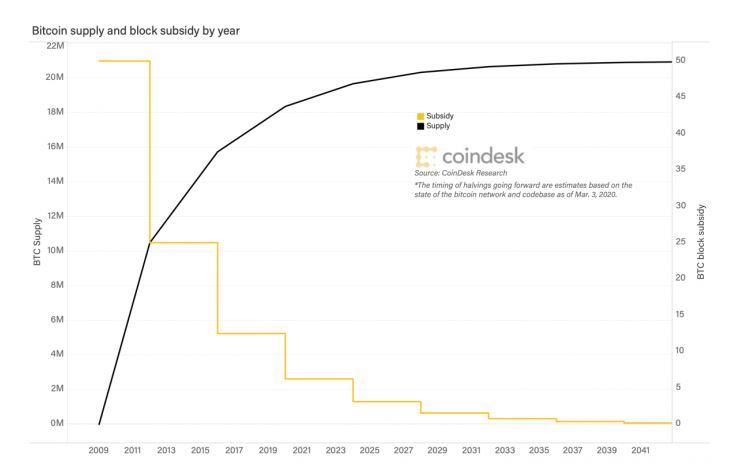
\includegraphics[width=0.6\linewidth]{Fig/05/F1}
    \caption{Bitcoin block reward in bitcoins. Figure sourced from  \href{https://www.coindesk.com/bitcoin-halving-explainer}{here}}
    \label{fig:f1}
\end{figure}

\begin{figure}[h!]
    \centering
    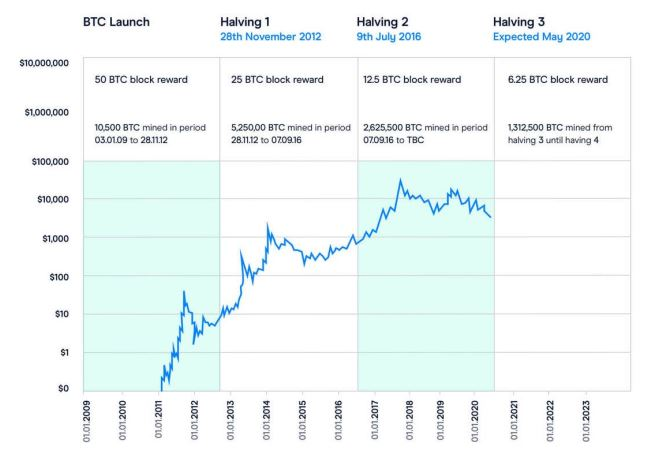
\includegraphics[width=0.6\linewidth]{Fig/05/F2}
    \caption{Bitcoin rewards in dollars. Figure sourced from  \href{https://www.cmcmarkets.com/en/learn-cryptocurrencies/bitcoin-halving}{here}}
    \label{fig:f2}
\end{figure}

The combination of coinbase transactions and transaction fees ensures the proper functioning and security of the Bitcoin network. Miners are motivated to continue mining, securing the network, and processing transactions as they receive both block rewards and transaction fees as incentives for their efforts. The gradual reduction in block rewards through halvings also creates a deflationary monetary policy, which further contributes to Bitcoin's scarcity and potential value appreciation over time (Figure \ref{fig:f1}, \ref{fig:f2}).

\subsection{Transaction mempool}
The transaction mempool plays a crucial role in the process of how Bitcoin transactions are propagated, verified, and eventually included in blocks. Here are the key points about the transaction mempool and its significance:
\begin{enumerate}
    \item \textbf{Transaction Propagation:}
    \begin{itemize}
        \item When a user wants to make a Bitcoin transaction, they create a transaction message, sign it using their private key, and broadcast it across the Bitcoin network.
        \item The transaction message is a few kilobytes in size and contains information about the transaction inputs, outputs, and the corresponding digital signatures.
        \item Miners in the network receive these transactions and verify the signatures before adding them to their memory pool, known as the "mempool."
    \end{itemize}
    \item \textbf{The Mempool:}
    \begin{itemize}
        \item The mempool is a temporary storage area where miners keep pending transactions that they have received and verified.
        \item Transactions in the mempool are waiting to be included in a block and added to the blockchain.
        \item Miners prioritize which transactions to include in their working block based on factors like the transaction fee rate (higher fee with smaller size).
    \end{itemize}
    \item \textbf{Block Size Limit:}
    \begin{itemize}
        \item Each block in the Bitcoin blockchain has a maximum size limit, currently set at 1 megabyte (MB) in the Bitcoin network.
        \item Miners aim to maximize the total transaction rewards in their block while adhering to this size limit.
    \end{itemize}
    \item \textbf{Transaction Fee Rates:}
    \begin{itemize}
        \item Miners prioritize transactions with higher transaction fees because they want to maximize their potential reward for including transactions in a block.
        \item Transactions with higher fees are more likely to be included in blocks sooner, incentivizing users to offer higher fees if they want their transactions processed quickly.
    \end{itemize}
    \item \textbf{Confirmation Latency:}
    \begin{itemize}
        \item There is a certain latency between the time a transaction is issued and when it is confirmed on the blockchain. This latency is influenced by two factors: (a) the time it takes for a transaction to be included in a block (which can be reduced by offering a higher transaction fee), and (b) the time it takes for that block to be buried deep enough in the longest chain for the transaction to be considered confirmed.
        \item Users may choose to trade off latency for security, deciding whether to use higher transaction fees for faster confirmation or lower fees for potentially longer confirmation times.
    \end{itemize}
    \item \textbf{Blockchain Design Trade-offs:}
    \begin{itemize}
        \item The trade-off between latency and security is specific to the Bitcoin blockchain design.
        \item Other blockchain designs may have different approaches and trade-offs, which will be explored in future lectures.
    \end{itemize}
\end{enumerate}
The mempool and the prioritization of transactions based on fees are essential components that allow the Bitcoin network to efficiently process and confirm transactions while incentivizing miners to maintain the security of the blockchain through the proof-of-work process (Figure \ref{fig:f3}).

\section{Validating a block}
\subsection{The state of the system}
The state of the blockchain system, also known as the UTXO set (Unspent Transaction Output set), is a critical component in ensuring the integrity of the cryptocurrency network. Here are the key points about the state of the system and its significance in Bitcoin:
\begin{enumerate}
    \item \textbf{Verifying Transaction Double-Spending:}
    \begin{itemize}
        \item One of the essential tasks in the Bitcoin system is to prevent double-spending, where a user attempts to spend the same coin or UTXO more than once.
        \item To verify the validity of a new transaction, users need to check if the transaction's inputs (UTXOs) have not been spent previously.
    \end{itemize}
    \item \textbf{Unspent Transaction Outputs (UTXOs):}
    \begin{itemize}
        \item The state of the system is represented by the set of UTXOs, which includes all transaction outputs that have not been spent in the blockchain.
        \item UTXOs are created when transactions are included in the blockchain and are considered valid until they are spent by new transactions.
    \end{itemize}
    \item \textbf{Separate from the Mempool:}
    \begin{itemize}
        \item The state of the system is distinct from the mempool, which contains pending transactions yet to be confirmed.
        \item The state consists of UTXOs that have been confirmed and permanently recorded in the blockchain.
    \end{itemize}
    \item \textbf{Role in Transaction Validation:}
    \begin{itemize}
        \item When miners construct new blocks from transactions in the mempool, they only include valid transactions by checking the information in the state (UTXO set).
        \item Transactions that attempt to spend already spent UTXOs are rejected as invalid.
    \end{itemize}
    \item \textbf{Summary of Ledger Entries:}
    \begin{itemize}
        \item The state contains a summary of all the confirmed ledger entries in the blockchain until the current point in time.
        \item This summary is crucial for validating new transactions and ensuring their consistency with previous transactions.
    \end{itemize}
    \item \textbf{Growth and Size Challenges:}
    \begin{itemize}
        \item The UTXO set grows over time as more transactions are confirmed and new UTXOs are created.
        \item As of now, the UTXO set size is quite large, over 5 GB, and it continues to increase as Bitcoin gains popularity.
        \item The size of the UTXO set presents scalability challenges, especially concerning memory requirements and specialized hardware for storage and management.
    \end{itemize}
\end{enumerate}
Overall, the state of the system (UTXO set) plays a vital role in maintaining the integrity of the Bitcoin network, preventing double-spending, and ensuring that new transactions are consistent with previous ones. Managing the growth of the UTXO set is an important aspect of addressing scalability concerns in the blockchain system.

\begin{figure}[h!]
    \centering
    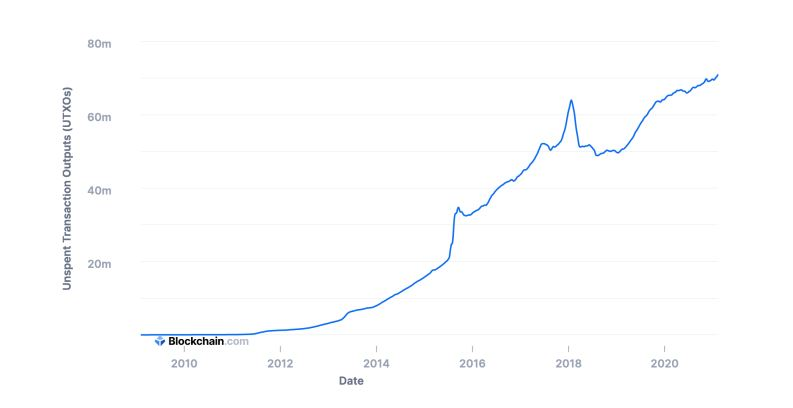
\includegraphics[width=0.6\linewidth]{Fig/05/F3}
    \caption{Number of UTXOs over time in Bitcoin. Figure sourced from \href{https://www.blockchain.com/explorer/charts/utxo-count}{here}}
    \label{fig:f3}
\end{figure}


\subsection{Validating blocks}
Validating blocks is a crucial step for miners in the Bitcoin network to ensure that the newly received or constructed block adheres to the rules and integrity of the blockchain. Here are the important points about block validation:

\begin{enumerate}
    \item \textbf{Proof-of-Work (PoW) Check:}
    \begin{itemize}
        \item The first check performed by a miner is to verify whether the proof of work presented in the block meets the required threshold.
        \item The proof-of-work is a computationally intensive puzzle that miners must solve to create a new block, and it ensures the security and immutability of the blockchain.
        \item If the proof-of-work is valid, the miner can proceed with further checks.
    \end{itemize}
    \item \textbf{Transaction Consistency Check:}
    \begin{itemize}
        \item After validating the proof-of-work, the miner needs to verify whether the transactions included in the block are consistent with the current state (UTXO set).
        \item This consistency check is crucial to prevent any attempts at double-spending or invalid transactions.
        \item The miner must confirm that each input in every transaction is a valid unspent transaction output (UTXO) according to the current state.
    \end{itemize}
    \item \textbf{Updating the State:}
    \begin{itemize}
        \item If all the transactions in the block pass the consistency check, the miner accepts the block, removes the relevant transactions from its mempool and updates the state (UTXO set).
        \item Updating the state involves deleting the spent transaction outputs (UTXOs) that were used as inputs in the block's transactions.
        \item Additionally, the newly generated unspent transaction outputs (UTXOs) are added to the state, representing the funds transferred in the block.
    \end{itemize}
    \item \textbf{Preemptive Validation in Block Construction:}
    \begin{itemize}
        \item Before a miner starts mining a new block, it performs the same validation steps preemptively on the transactions it intends to include in the block.
        \item This ensures that the constructed block will be accepted by the network once it is mined, saving computational effort.
    \end{itemize}
\end{enumerate}
In summary, block validation is a critical process to maintain the integrity of the blockchain. Miners verify the proof-of-work and the consistency of transactions with the current state (UTXO set). Once validated, a new block is added to the blockchain and the state is updated to reflect the changes made by the included transactions.
\subsection{Light nodes and stateless clients}
Light nodes and stateless clients are important concepts in blockchain networks, especially for enhancing scalability and allowing users with limited resources to participate in the system. Here's an explanation of these concepts:
\begin{enumerate}
    \item \textbf{Light Nodes / Light Clients:}
    \begin{itemize}
        \item Light nodes, also known as light clients, are participants in the blockchain network who do not store the full state of the system.
        \item Instead, they only verify the proof-of-work on blocks to ensure their validity, and they may selectively verify specific transactions that concern them.
        \item By avoiding the storage of the entire state, light nodes require much less computation and storage power compared to full nodes, making them more accessible to devices with limited resources.
    \end{itemize}
    \item \textbf{Stateless Clients:}
    \begin{itemize}
        \item Stateless clients are an extension of light nodes that aim to validate transactions and blocks without maintaining the full state of the blockchain at all times.
        \item Instead of storing the entire state, stateless clients download only the necessary state information on-demand to validate a specific block or transaction.
        \item Once the validation is complete, the stateless client can delete the downloaded state information to save storage space.
        \item To securely handle the state information, it is stored in the form of an accumulator, a data structure that we discussed in Lecture 2 of the blockchain course.
    \end{itemize}
    \item \textbf{Advantages of Stateless Clients:}
    \begin{itemize}
        \item The adoption of stateless clients can significantly enhance the scalability of blockchain networks. It allows more users to participate without the need for extensive resources to store the full state.
        \item By reducing the storage requirements for clients, the network becomes more inclusive and accessible to a wider range of devices, including mobile phones and low-powered computers.
        \item Stateless clients can still contribute to the network's security by validating transactions and blocks, albeit without maintaining a persistent copy of the state.
    \end{itemize}
    \item \textbf{Implementation in Ethereum:}
    \begin{itemize}
        \item The concept of stateless clients is actively pursued by the Ethereum blockchain network as a scalability solution.
        \item Ethereum aims to transition from a stateful design (where clients store the full state) to a stateless design, using stateless clients to improve the network's performance and reduce resource requirements.
    \end{itemize}
\end{enumerate}
In conclusion, light nodes and stateless clients are innovative approaches to make blockchain networks more scalable and inclusive. By allowing participants to interact with the network without storing the full state, these concepts address the challenges of resource-intensive storage and computation in traditional blockchain architectures.

\section{Smart contracts}
In the context of blockchain technology, smart contracts are self-executing contracts with the terms and conditions written directly into code. They are programmed to automatically execute and enforce the terms of the contract without the need for a trusted third party. Smart contracts run on blockchain networks, and their execution is validated and recorded on the blockchain, making them transparent and immutable.\\
In traditional settings, when two parties want to exchange money subject to certain conditions, they create a written contract and rely on a trusted intermediary or authority to enforce the contract's terms. With smart contracts on a blockchain, this intermediary is eliminated, and the trust is decentralized across the network.\\
In summary, smart contracts are a powerful innovation that leverages blockchain technology to enable secure, automated, and transparent execution of agreements without the need for intermediaries. While Bitcoin's smart contract capabilities are limited, other blockchain platforms like Ethereum have expanded the possibilities of smart contracts to revolutionize various industries and applications.
\subsection{Scripts in Bitcoin}
In the context of Bitcoin, smart contracts are referred to as "scripts." A script is a sequence of opcodes included in every transaction output, specifying the conditions that must be satisfied to spend the coins from that output. By using different combinations of opcodes, Bitcoin scripts can enforce various conditions beyond the default ones, providing a level of programmability.

The default condition in a regular transaction output requires the spender to provide a public key that matches the address mentioned in the output and sign the transaction with the corresponding private key. This ensures that only the rightful owner of the coins can spend them.

However, Bitcoin scripts allow for additional conditions to be specified. Some examples include:
\begin{enumerate}
    \item \textbf{Timelocks:} A transaction can be configured to be unspendable until a certain block height or a specific time is reached. This can be useful for time-sensitive transactions or implementing time-based conditions.
    \item \textbf{Multisig:} A script can require multiple signatures from different private keys to spend the coins. This allows for escrow-like arrangements, where funds are held until all parties involved in the transaction provide their signatures.
    \item \textbf{Hashed Timelock Contracts (HTLCs):} HTLCs are a specific type of smart contract that combines time locks and hash locks. They are useful for setting up secure escrow arrangements for exchanging assets or payments between parties, ensuring that both parties fulfill their obligations before the funds are released.
\end{enumerate}
The combination of these conditions in Bitcoin scripts enables the creation of more sophisticated smart contracts, even though Bitcoin's scripting language is not as powerful as the one used in platforms like Ethereum. While Bitcoin's script language is intentionally limited for security reasons, it still provides enough flexibility to implement useful smart contract functionalities, especially for simple financial transactions and basic programmability.
